\documentclass[landscape]{slides}
\usepackage[landscape]{geometry}
\usepackage{amsmath}
\usepackage[pdftex]{graphicx}
\title{A new set of sigma/Quadrature points for a Gaussian PDF that can capture all 4th and 6th moments "exactly"}
\author{Nagavenkat Adurthi}
\date{\today}
\begin{document}
\maketitle
\normalsize

%********--------*****-----------********---------
\begin{slide}
{\bf From the basics}\newline\newline
Consider a discrete dynamic system with noise
\begin{align*}
x_{k+1}=f(x_k,k)+\nu_k
\end{align*}
	The PDF of this dynamic system propagates according to the {\bf Chapman Kolmogorov Equation}.
	\begin{align*}
	P(x_{k+1})=\int{P(x_{k+1}|x_k)P(x_k)}dx_k
	\end{align*}
	\end{slide}
		%********--------*****-----------********---------
\begin{slide}
	$\bullet$ $P(x_k)$ in the CKE need not be gaussian at all times even though the initial condition was gaussian. \newline\newline
	$\bullet$ It would be gaussian at all time only when system is linear and the noise is also gaussian. In this case it is very easy to {\bf solve this equation analytically}.\newline \newline
	Incase the  the system in nonlinear and noise is gaussian, the CKE would be
	\begin{align*}
	P(x_{k+1})=\int{{\bf\emph{N}}(x_{k+1}|x_k)P(x_k)}dx_k
	\end{align*}\newline
	\end{slide}
		%********--------*****-----------********---------
\begin{slide}
	{\bf Extended Kalman Filter}\newline\newline
	$P(x_k)$ is not always gaussian and there is no analytical solution to this equation. Hence the EKF emerged that can provide an {\bf analytical solution} to this CKE by considering the following {\bf two approximations}\newline\newline
	$\bullet$ $P(x_k)$ is replaced by an equivalent gaussian PDF that has the same first two moments as the original PDF $P(x_k)$.\newline\newline
	$\bullet$ $f(x_k,k)$ is linearized in ${\bf\emph{N}}(x_{k+1}|x_k)$.
	\end{slide}
	\begin{slide}
	$\bullet$ The EKF works well for systems in which the linearized dynamics is a good approximation to the nonlinear system.- {\bf Higher order terms in Taylor series are negligible}.\newline\newline 
	$\bullet$ If the nonlinearity is too strong the EKF would diverge. \newline\newline
	$\bullet$ Above that during the linearization process the computation of the jacobian is {\bf computationally expensive}. \newline\newline
	$\bullet$ The EKF {\bf disregards the actual state PDF} and propagates only the first two moments of the state PDF. The linearized dynamics are used in the propagation of the first two moments.
		\end{slide}
		%********--------*****-----------********---------
\begin{slide}
Propagation of mean
\begin{align*}
\mu_{k+1}=f(\mu_k)\\
\end{align*}
Propagation of Covariance
\begin{align*}
P_{k+1}=AP_kA^T+Q_k\\
\end{align*}
Where A is the jacobian of the system.
\begin{align*}
A=\frac{\partial{f}}{\partial{x}}|_{\mu_k}
\end{align*}
	\end{slide}
		%********--------*****-----------********---------
\begin{slide}

 {\bf Linear Regression Kalman Filter - LRKF}\newline \newline
	$\bullet$ The LRKF also uses linearized dynamics but the linearization is not done using the taylor series (hence evaluating jacobian) but by a method called {\bf statistical linearization}.\newline \newline 
	$\bullet$ Firstly sample points are chosen about the current mean at time $k$ such that the mean of the samples and covariance of the samples {\bf match} the current mean and current covariance.\newline \newline 
	$\bullet$ Each point is propagated using the {\bf nonlinear dynamics} of the system to time step $k+1$.\newline \newline
	$\bullet$ Now between the current sample points at time $k$ and the corresponding propagated points at time $k+1$ a {\bf linear model is fit} which gives rise to the linearized dynamics of the system at time $k$.\newline \newline
	$\bullet$ Now this linearized dynamics is used to compute the mean and covariance at time step $k+1$. 
		\end{slide}
		%********--------*****-----------********---------
\begin{slide}
	The sample points at time $k$  are 
\begin{align*}
\mu_k&=\frac{1}{n}\sum_{i=1}^{N}X^i\\
P_k&=\frac{1}{n}\sum_{i=1}^{N}(X^i-\mu_k)(X^i-\mu_k)^T
\end{align*}
And now each sample point is individually propagated using nonlinear dynamics
\begin{align*}
Y^i=f(X^i)
\end{align*} 
	\end{slide}
		%********--------*****-----------********---------
\begin{slide}	 
Now trying to fit a linear model between the points $(Y^i,X^i)$
\begin{align*}
Y=AX+B
\end{align*}
This is standard linear fit procedure by minimizing the least square error
\begin{align*}
e_i&=Y^i-AX^i-B\\
E&=(e_i)^T(e_i)
\end{align*}
The mean and covariance at time $k+1$ can be found from the Kalman filter propagation equations
	\begin{align*}
\mu_{k+1}&=A\mu_k\\
P_{k+1}&=AP_kA^T+Q_k
\end{align*}
	\end{slide}
		%********--------*****-----------********---------
\begin{slide}

 {\bf Unscented Kalman Filter- Unscented Transform}\newline\newline
 $\bullet$The UKF works in the same ways as the LRKF but the samples are chosen in a {\bf determined} way such that they always match the mean and covariance or higher moments at the current step.\newline\newline
 $\bullet$ The points are propagated using the {\bf nonlinear dynamics}. The mean and covariance at time step $k+1$ are calculated from these propagated points.\newline\newline
 $\bullet$ The {\bf first approximation} the UKF does to the CKE is that it replaces the current state PDF with a gaussian PDF with same first two moments. \newline\newline
 $\bullet$ There is {\bf no linearizations involved}, instead the integral is itself evaluated approximately using quadrature points of the gaussian weighting function-{\bf second approximation}.\newline\newline
  $\bullet$ The UKF like the EKF only keeps track of the first two moments of the state PDF.\newline\newline
  $\bullet$ We can still improve the {\bf second approximation} by better evaluating the integrals.
 	\end{slide}
		%********--------*****-----------********---------
\begin{slide}
 One could look at the UKF in the following perspective, starting from CKE
\begin{align*}
	P(x_{k+1})=\int{{\bf\emph{N}}(x_{k+1}|x_k)P(x_k)}dx_k
	\end{align*}
		Replacing the state PDF with gaussian pdf with equivalent mean $\mu_k$ and covariance $P_k$. 
		\begin{align*}
	P(x_{k+1})=\int{{\bf\emph{N}}(x_{k+1}|x_k){\bf\emph{N}}(x_k)}dx_k
	\end{align*}
	Calculating the mean of $P(x_{k+1}$ by integrating on both side wrt $x_{k+1}$.
		\begin{align*}
	\mu_{k+1}&=\int{\int{{\bf\emph{N}}(x_{k+1}-f(x_k)|Q_k)}dx_{k+1}{\bf\emph{N}}(x_k)}dx_k\\
	&=\int{f(x_k){\bf\emph{N}}(x_k)}dx_k
	\end{align*}
		\end{slide}
		%********--------*****-----------********---------
\begin{slide}
The covariance can be calculated from the second raw moment
			\begin{align*}	E[x_{k+1}x_{k+1}^T]&=\int{\int{x_{k+1}x_{k+1}^T{\bf\emph{N}}(x_{k+1}-f(x_k)|Q_k)}dx_{k+1}{\bf\emph{N}}(x_k)}dx_k\\
	&=\int{(f(x_k)f(x_k)^T+Q_k){\bf\emph{N}}(x_k)}dx_k
	\end{align*}
	By parallel axis theorem for moments the covariace is calculated as
	\begin{align*}
	P_k&=E[x_{k+1}x_{k+1}^T]-\mu_{k+1}\mu_{k+1}^T
	\end{align*}
	$\bullet$Thus by evaluating two integrals we get the mean and covariance.\newline\newline
	$\bullet$ The second raw moment and the mean need to be evaluated accurate enough or else the parallel axis theorem for moments might render the {\bf {\emph covariance to be positive semi definite}}.
		\end{slide}
		%********--------*****-----------********---------
\begin{slide}
	For example in a 1D case, the integrals would be
	 \begin{align*}
	 \mu_{k+1}&=\int{f(x_k){\bf\emph{N}}(x_k)}dx_k\\
	 &=\sum_{i=1}^{N}w^if(x_k^i)\\
	E[x_{k+1}^2]&=\int{(f(x_k)^2+Q_k){\bf\emph{N}}(x_k)}dx_k\\
	&=\sum_{i=1}^{N}w^if(x_k^i)^2+Q_k\sum_{i=1}^{N}w^i\\
	&=\sum_{i=1}^{N}w^if(x_k^i)^2+Q_k
	\end{align*}
	The covariance is
	\begin{align*}
	P_k&=E[x_{k+1}^2]-\mu_{k+1}^2\\
	&=\sum_{i=1}^{N}w^i(f(x_k^i)-\mu_{k+1})^2
	\end{align*} 
	Thus the UKF boils down to just evaluating the integrals involving gaussian kernel using the quadrature points.
		\end{slide}
		%********--------*****-----------********---------
\begin{slide}
 {\bf Unscented Transform-Integration using Quadrature points for Gaussian Kernel}\newline\newline
	$\bullet$ This section shows the derivation of a new set of quadrature points that can exactly match all the first four and even six moments of the gaussian weighting function for any dimension. \newline\newline
	$\bullet$ The main {\bf draw back} of the $2n+1$, $4n+1$ or even the $6n+1$ sigma points is that they cannot capture the 4th moment or any higher order even moment exactly. It is illustrated that {\bf we need to search in additional directions} to satisfy higher order moments.\newline\newline
	$\bullet$ An example is presented that evidently shows that these methods cannot capture the 4th moment of the gaussian weigting function.
	\end{slide}
		%********--------*****-----------********---------
\begin{slide}
{\bf An Example illustrating the fact that the $2n+1$, $4n+1$ and $6n+1$ set of sigma points cannot satisfy the 4th moment}\newline\newline
$\bullet$ All these set of sigma points tend to pick symmetric points on the principle axis of the $\sigma$ contours.\newline\newline
$\bullet$ Their distances from the mean and the corresponding weights are chosen in a heuristic manner such that they satisfy the covariances.\newline\newline 
$\bullet$The main motive is that we have a gaussian pdf and we want to discretize it such that the discrete pdf can capture the moments of the continuous gaussian pdf. 
		\end{slide}
		%********--------*****-----------********---------
\begin{slide}
	For example consider a 2D system.The square root of the covariance matrix P is defined as 
\begin{align*}
\sqrt{P}&=AA^T
\end{align*}
where A is the matrix square root. Let	
\[P=\left[ {\begin{array}{cc}
 P_{11} & P_{12}  \\
 P_{12} & P_{22}  \\
 \end{array} } \right]\]
if A is considered to be the principle square root of the symmetric matrix P then A is also symmetric. \newline
\[A=\left[ {\begin{array}{cc}
 \sigma_{11} & \sigma_{12}  \\
 \sigma_{12} & \sigma_{22}  \\
 \end{array} } \right]\]
 	\end{slide}
		%********--------*****-----------********---------
\begin{slide} 
 \begin{align*}
 P_{11}&=\sigma_{11}^2+\sigma_{12}^2\\
 P_{12}&=\sigma_{11}\sigma_{12}+\sigma_{12}\sigma_{22}\\
 P_{22}&=\sigma_{12}^2+\sigma_{22}^2
 \end{align*}
 The priciple axis of the $1\sigma$ contour are columns of A i.e.
 \[\sigma_1=\left[ {\begin{array}{c}
 \sigma_{11}  \\
 \sigma_{12}  \\
 \end{array} } \right]\]
 and
  \[\sigma_2=\left[ {\begin{array}{c}
 \sigma_{12}  \\
 \sigma_{22}  \\
 \end{array} } \right]\]
 	\end{slide}
		%********--------*****-----------********---------
\begin{slide}
 $\bullet$ Now for example the $4n+1$ set of sigma points for the 2D case has 1 point on the mean, 4 points on the principle axis of  $r_1\sigma$ contour and the rest 4 points on the principle axis of another $r_2\sigma$ contour.\newline\newline 
 $\bullet$ The mean is considered as the origin as once the points are found they can be translated by the given mean vector. \newline\newline
 $\bullet$ The points that lie on the same contour have the same weights. So now there are only 3 weights:  $w_0$ for the mean, $w_1$ for the 4 $r_1\sigma$ contour points and $w_2$ for the 4 $r_2\sigma$ contour points. 
 \end{slide}
 %********-------------*********
 \begin{slide}
 The points are
 \begin{align*}
 &(0,0)\\
 &(r_1\sigma_{11},r_1\sigma_{12})\\
 &(-r_1\sigma_{11},-r_1\sigma_{12})\\
 &(r_1\sigma_{12},r_1\sigma_{22})\\
 &(-r_1\sigma_{12},-r_1\sigma_{22})\\
 &(r_2\sigma_{11},r_2\sigma_{12})\\
 &(-r_2\sigma_{11},-r_2\sigma_{12})\\
 &(r_2\sigma_{12},r_2\sigma_{22})\\
 &(-r_2\sigma_{12},-r_2\sigma_{22})
 \end{align*}
   	\end{slide}
		%********--------*****-----------********---------
\begin{slide}
 Visually they look like \newline
 %******************
\begin{figure}
	\centering
		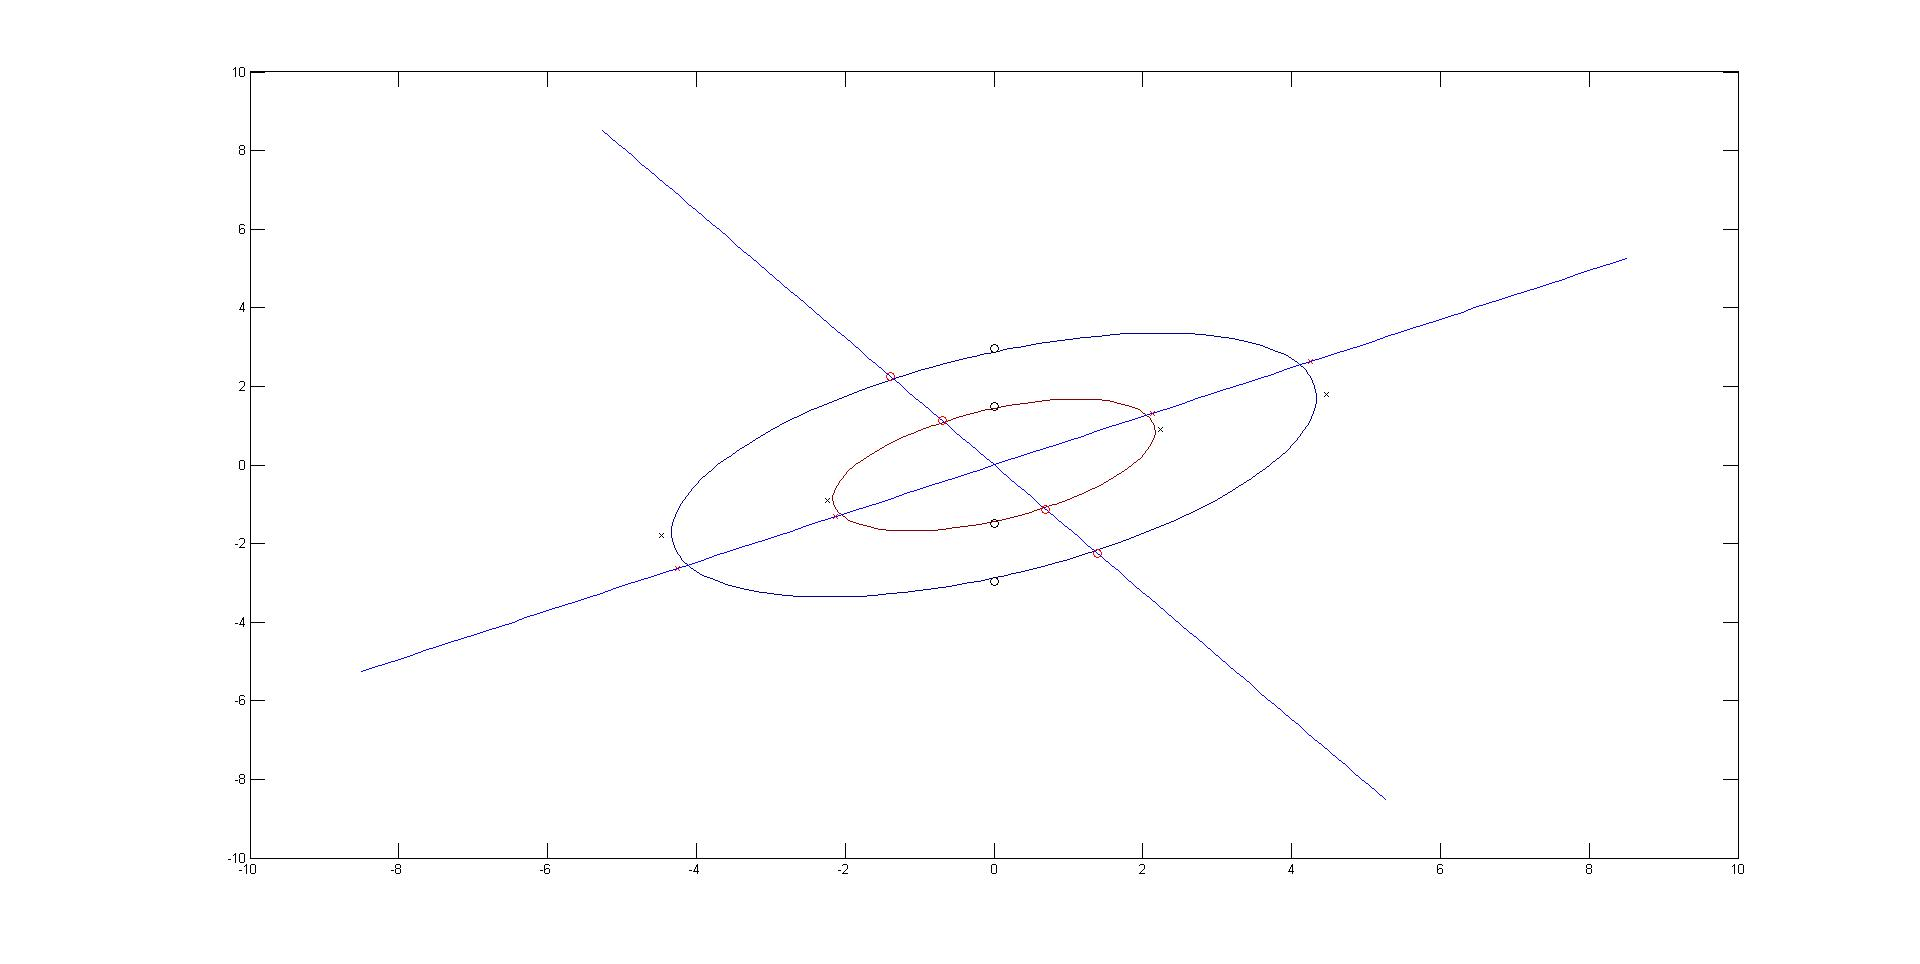
\includegraphics[width=0.8\textwidth]{4np1pts.jpg}
	\label{fig:4np1pts}
\end{figure}\newline
 %******************
 $\bullet$ There are two sets of points on each sigma contour. This is just to illustrate the difference between the points derived from principle square root and cholesky decomposition of P. \newline
 $\bullet$Cholesky decomposition results in points that lie on the ellipse/ contour but not on the principle axis.
    	\end{slide}
		%********--------*****-----------********---------
\begin{slide}
 $\bullet$The mean and all {\bf higher order odd moments} are automatically satisfied as the points are chosen to be {\bf symmetric}.\newline 
 The covariance equations i.e. the second moments are
\begin{align*} 
E[x_1^2]&=\sum{w_ix_{1i}^2}=(2w_1r_1^2+2w_2r_2^2)(\sigma_{11}^2+\sigma_{12}^2)=P_{11}\\ E[x_1x_2]&=\sum{w_ix_{1i}x_{2i}}=(2w_1r_1^2+2w_2r_2^2)(\sigma_{11}\sigma_{12}+\sigma_{12}\sigma_{22})=P_{12}\\
E[x_2^2]&=\sum{w_ix_{2i}^2}=(2w_1r_1^2+2w_2r_2^2)(\sigma_{12}^2+\sigma_{22}^2)=P_{22}
 \end{align*} 
 $\bullet$ It can be seen that by choosing points on the sigma contours the 3 equations for a 2D case collapse into just solving one equations i.e.
 \begin{align*}
 2w_1r_1^2+2w_2r_2^2&=1
 \end{align*}
    	\end{slide}
		%********--------*****-----------********---------
\begin{slide}
 Now looking at the 4th moment.
 \tiny
 \begin{align*}
  E[x_1^4]&=\sum{w_ix_{1i}^4}=(2w_1r_1^4+2w_2r_2^4)(\sigma_{11}^4+\sigma_{12}^4)\equiv 3P_{11}^2\\ E[x_1^3x_2]&=\sum{w_ix_{1i}^3x_{2i}^2}=(2w_1r_1^4+2w_2r_2^4)(\sigma_{11}^3\sigma_{12}+\sigma_{12}^3\sigma_{22})\equiv3P_{11}P_{12}\\
E[x_1^2x_2]&=\sum{w_ix_{1i}^2x_{2i}^2}=(2w_1r_1^4+2w_2r_2^4)(\sigma_{11}^2\sigma_{12}^2+\sigma_{12}^2\sigma_{22}^2)\equiv P_{11}P_{22}+2P_{12}^2\\
E[x_1^1x_2^3]&=\sum{w_ix_{1i}x_{2i}^3}=(2w_1r_1^4+2w_2r_2^4)(\sigma_{11}\sigma_{12}^3+\sigma_{12}\sigma_{22}^3)\equiv 3P_{22}P_{12}\\
E[x_2^4]&=\sum{w_ix_{2i}^4}=(2w_1r_1^4+2w_2r_2^4)(\sigma_{12}^4+\sigma_{22}^4)\equiv 3P_{22}^2\\ 
 \end{align*}
 \normalsize
$\bullet$Here we have 5 equations which seem to have the same left hand side of variables $2w_1r_1^4+2w_2r_2^4$ but different right hand side of constant values.\newline\newline 
$\bullet$These are like {\bf parallel curves} that do not intersect and cannot be solved for. It does not matter how many points we take on the principle axis or in general sigma contour formed from $\sqrt{P}$, we always end up in the above structure. 
   	\end{slide}
		%********--------*****-----------********---------
\begin{slide}
{\bf Searching for Quadrature points on principle axis and conjugate axis that can satisfy the 4th moment "`exactly"}\newline
	 Again for a 2D case, the axis are chosen as\newline
	Principle axis:
\[\sigma_1=\left[ {\begin{array}{c}
 \sigma_{11}\\
 \sigma_{12}
 \end{array} } \right]\]
 \[\sigma_2=\left[ {\begin{array}{c}
 \sigma_{12}\\
 \sigma_{22}
 \end{array} } \right]\]
 Conjugate axis:
 \begin{align*}
 \sigma_3=\sigma_1+\sigma_2\\
 \sigma_4=\sigma_1-\sigma_2
 \end{align*}
    	\end{slide}
		%********--------*****-----------********---------
\begin{slide}
 The points are therefore
  \begin{align*}
 &(0,0)\\
 &(r_1\sigma_{11},r_1\sigma_{12})\\
 &(-r_1\sigma_{11},-r_1\sigma_{12})\\
 &(r_1\sigma_{12},r_1\sigma_{22})\\
 &(-r_1\sigma_{12},-r_1\sigma_{22})\\
 &(r_2(\sigma_{11}+\sigma_{12}),r_2(\sigma_{12}+\sigma_{22}))\\
 &(-r_2(\sigma_{11}+\sigma_{12}),-r_2(\sigma_{12}+\sigma_{22}))\\
 &(r_2(\sigma_{11}-\sigma_{12}),r_2(\sigma_{12}-\sigma_{22}))\\
 &(-r_2(\sigma_{11}-\sigma_{12}),-r_2(\sigma_{12}-\sigma_{22}))
 \end{align*}
    	\end{slide}
		%********--------*****-----------********---------
\begin{slide}
 Visually they look like \newline\newline
 %******************
\begin{figure}
	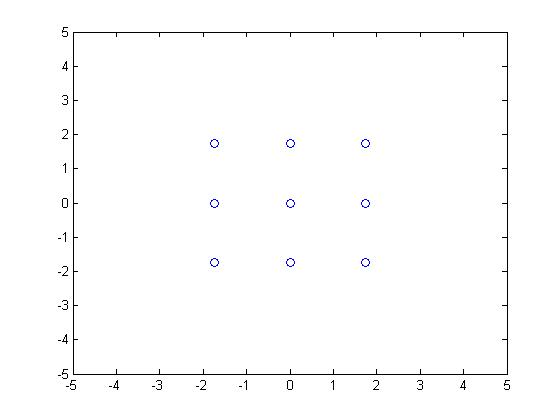
\includegraphics[width=0.5\textwidth]{eye2quadpts.jpg}
	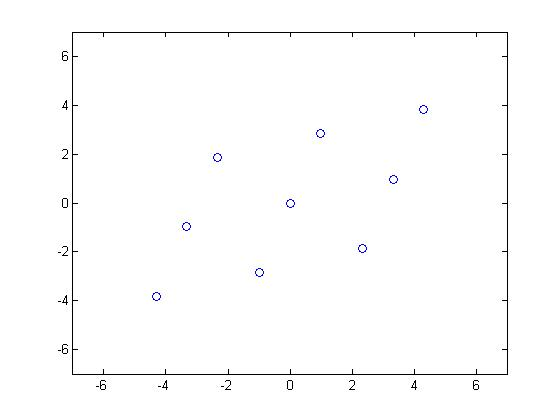
\includegraphics[width=0.5\textwidth]{P2Dquadpts.jpg}
	\caption{(a)Indentity Cov and (b)$[4,2;2,3]$ Cov}
	\label{fig:eye2quadpts}
\end{figure}
 %******************
    	\end{slide}
		%********--------*****-----------********---------
\begin{slide}
{\bf Isserlis Theorem}:\newline\newline
 Any arbitrary moment of a Gaussian PDF is given by 
 \begin{align*}
 E[x_1x_2x_3....x_{2n}]=\sum\prod{E[x_ix_j]}
 \end{align*} 
 for example the fourth moment is
 \begin{align*}
 E[x_1x_2x_3x_4]=E[x_1x_2]E[x_3x_4]+E[x_1x_3]E[x_4x_5]+E[x_1x_4]E[x_2x_3]
 \end{align*}
 Therefore any order moment higher than 2 is dependent on the entries of the covariance matrix
    	\end{slide}
		%********--------*****-----------********---------
\begin{slide}
 The 2nd moment equations are
 \begin{align*} 
E[x_1^2]&=\sum{w_ix_{1i}^2}=(2w_1r_1^2+4w_2r_2^2)(\sigma_{11}^2+\sigma_{12}^2)=P_{11}\\ E[x_1x_2]&=\sum{w_ix_{1i}x_{2i}}=(2w_1r_1^2+4w_2r_2^2)(\sigma_{11}\sigma_{12}+\sigma_{12}\sigma_{22})=P_{12}\\
E[x_2^2]&=\sum{w_ix_{2i}^2}=(2w_1r_1^2+4w_2r_2^2)(\sigma_{12}^2+\sigma_{22}^2)=P_{22}
 \end{align*} 
 From these 3 equations we are only left to solve the equation
 \begin{align*}
 2w_1r_1^2+4w_2r_2^2=1
 \end{align*}
 Now if we consider the 5- 4th order moment equations 
% \begin{align} E[x_1^4]&=\sum{w_ix_{1i}^4}=(2w_1r_1^4+2w_2r_2^4)(\sigma_{11}^4+\sigma_{12}^4)\equiv 3P_{11}^2\\ %E[x_1^3x_2]&=\sum{w_ix_{1i}^3x_{2i}^2}=(2w_1r_1^4+2w_2r_2^4)(\sigma_{11}^3\sigma_{12}+\sigma_{12}^3\sigma_{22})\equiv3P_{11}P_{12}\\
%E[x_1^2x_2]&=\sum{w_ix_{1i}^2x_{2i}^2}=(2w_1r_1^4+2w_2r_2^4)(\sigma_{11}^2\sigma_{12}^2+\sigma_{12}^2\sigma_{22}^2)\equiv P_{11}P_{22}+2P_{12}^2\\
%E[x_1^1x_2^3]&=\sum{w_ix_{1i}x_{2i}^3}=(2w_1r_1^4+2w_2r_2^4)(\sigma_{11}\sigma_{12}^3+\sigma_{12}\sigma_{22}^3)\equiv 3P_{22}P_{12}\\
%E[x_2^4]&=\sum{w_ix_{2i}^4}=(2w_1r_1^4+2w_2r_2^4)(\sigma_{12}^4+\sigma_{22}^4)\equiv 3P_{22}^2\\ 
% \end{align}
 we are only left to solve the 2 equations
  \begin{align*}
 2w_1r_1^4+4w_2r_2^4&=3\\
 4w_2r_2^4&=1
 \end{align*}
 \end{slide}
 %***************----------**********--------------
 \begin{slide}
 Now if we apply the same procedure to n-dimensional system we can generalise the set of equations. In summary 
 \begin{align*}
 2w_1r_1^2+2^nw_2r_2^2&=1\\
  2w_1r_1^4+2^nw_2r_2^4&=3\\
 2^nw_2r_2^4&=1\\
 w_0=1-2nw_1-2^nw_2
 \end{align*} 
 equations have to be solved for $w_1,r_1,w_2,r_2$. In total there are {\bf $2n+2^n+1$} points.1 point of weight $w_0$ on the mean, $2n$ points of weight $w_1$ lie on the principle axis on the $r1\sqrt{P}$ contour, rest $2^n$ points lie on the conjugate axis symmetrically. \newline\newline
   	\end{slide}
		%********--------*****-----------********---------
\begin{slide}
{\bf Results of integration compared to Gauss Hermite integration for 3D system}\newline\newline
Here in this section the new set of quadrature points for 3D case are put to test, {\bf compared to gauss hermite integration}. As the new set of points are only {\bf good till fourth moment} we would consider the integration of {\bf polynomials till degree 4}.\newline
\[
 P = \begin{bmatrix}
       4 & 2 & 1    \\
       2 & 9 & 1     \\
       1 & 1 & 16
     \end{bmatrix}
\]
\begin{align*}
F&=x_1^4+x_2^4+x_3^4+x_1^3x_2+x_1^2x_2^2+\\
 &+x_3^2x_2^2+x_1^2x_3^2+x_1^3x_3+x_2^3x_3+x_3^3x_2
\end{align*}
\tiny
\begin{center}
  \begin{tabular}{ | l | l | l | l | l | }
    \hline
       No. of pts 					& $2^3=$ 8 							& $3^3=$ 27 			  & $4^3=$ 64			 & $10^3=$ 1000 (Truth) \\ \hline 
      GH          					&   1056.95571  			  & 1797.9999999      & 1798.00     	 &   1798.00           \\ \hline
\% error wrt Truth       	  &   41.2149211    			&  4.299e-013  	  	& 3.03502e-013   &   0         \\ 
      \hline
  \end{tabular}
\end{center} 

\begin{center}
  \begin{tabular}{ | l | l | l | l | l | }
    \hline
                  					&   No. of pts			& Integration result 			  & \% error wrt Truth			 \\ \hline 
      NM          					&   15       			  & 1797.99999998858          & 6.355208041935254e-010   \\
      \hline
  \end{tabular}
\end{center}
   	\end{slide}
		%********--------*****-----------********---------
\begin{slide}
{\bf Quadrature points to capture the 6th moment exactly }\newline
$\bullet$ To capture the 6th order moments exactly extra points are taken on different set of axis.\newline
$\bullet$ For example consider the 3D case. There are 3 principle axis $\sigma_1$, $\sigma_2$ and $\sigma_3$. Additional axis that are {\bf constructed from these axis} are\newline
The principle axis have 6 points
 \begin{align*}
 (\sigma_1,
 \sigma_2,
 \sigma_3)
 \end{align*}
The conjugate axis have 8 points
\begin{align*}
\sigma_1+\sigma_2+\sigma_3\\
\sigma_1-\sigma_2+\sigma_3\\
\sigma_1+\sigma_2-\sigma_3\\
\sigma_1-\sigma_2-\sigma_3
\end{align*}   	
\end{slide}
		%********--------*****-----------********---------
\begin{slide}
The new axis lie in each of the orthogonal planes, pass through the origin and are $45^o$ to each axis in that plane. There are 12 pts on these axis
\begin{align*}
\sigma_1+\sigma_2\\
\sigma_1-\sigma_2\\
\sigma_1+\sigma_3\\
\sigma_1-\sigma_3\\
\sigma_2+\sigma_3\\
\sigma_2-\sigma_3
\end{align*}
 In total there are $6+8+12=26$ quadrature points to capture all the 6th order and lower moments.
    	\end{slide}
		%********--------*****-----------********---------
\begin{slide} 
%*******************
%\begin{figure}
	\centering
		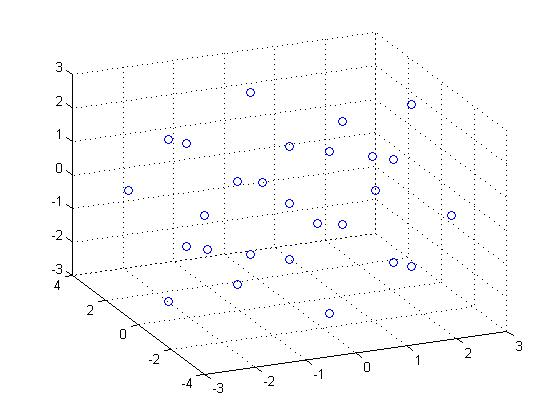
\includegraphics[width=0.92\textwidth]{3d6thmomentpts.jpg}
	\label{fig:3d6thmomentpts}
%\end{figure}
\newline
 %******************
%\begin{center}
	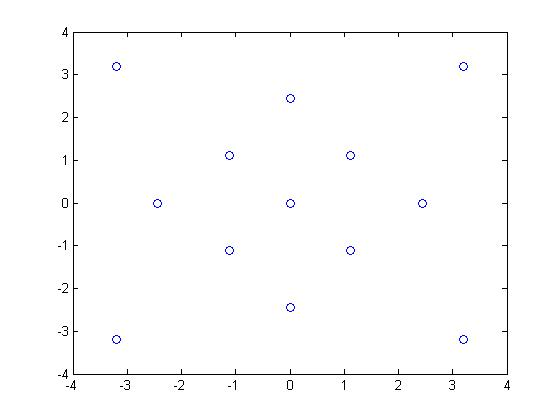
\includegraphics[width=0.92\textwidth]{2dcorr6thmomentpts.jpg}
	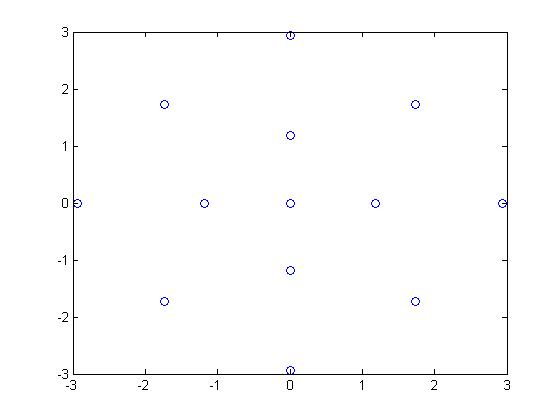
\includegraphics[width=0.92\textwidth]{2d_weird_case2.jpg}
	\label{fig:eye2quadpts}
%\end{center}
 %******************
\end{slide}
		%********--------*****-----------********---------
\begin{slide}
 For a general n- Dimensional system the equations to be solved a
 \begin{align*}
 2r_1^2w_1+2^nr_2^2w_2+4(n-1)r_3^2w_3&=1\\
 2r_1^4w_1+2^nr_2^4w_2+4(n-1)r_3^4w_3&=3\\
 2^nr_2^4w_2+4r_3^4w_3&=1\\
 2r_1^6w_1+2^nr_2^6w_2+4(n-1)r_3^6w_3&=15\\
 2^nr_2^6w_2+4r_3^6w_3&=3\\
 2^nr_2^6w_2&=1
 \end{align*}
 There are in total {\bf $2n+2^n+2n(n-1)$} points.
    	\end{slide}
		%********--------*****-----------********---------
\begin{slide}
 {\bf Results of integration compared to Gauss Hermite integration for 4D system}\newline\newline
Here in this section the new set of quadrature points to capture the 6th moment also for {\bf 4D case} are put to test, compared to {\bf gauss hermite quadrature points}. As the new set of points are only {\bf good till sixth order moment} we would consider the integration of polynomials till {\bf degree 6}.\newline
 The covariance of the gaussian Kernel
\[
 P = \begin{bmatrix}
       4 & 1 & 2  & 1   \\
       1 & 9 & 2  & 3   \\
       2 & 2 & 16 & 4  \\
       1 & 3 & 4 & 25  
     \end{bmatrix}
\]
\begin{align*}
F&=x_1^6+x_2^6+x_3^6+x_4^6+x_1^4+x_2^4+x_3^4+x_4^4+x_1^2x_2^2x_3^2+\\
&+x_1^3x_3+x_1^2x_2^4+x_3^4x_2^2+x_1^2x_3^4+x_1^3x_3+x_2^3x_3+x_3^3x_2
\end{align*}
\tiny
%\begin{table}
  \begin{tabular}{ | l | l | l | l | l | l | }
    \hline
       No. of pts 					& $2^4=$ 16 							& $3^4=$ 81 			  & $4^4=$ 256			 & $5^4=$ 64 	  	& $20^4=$ 160000 \\ \hline 
      GH          					&   84462.6354  		& 293311.8446    & 375417.9999     	 & 375417.9999  		  &   375417.9999           \\ \hline
\% error        	  &   77.5017    		&  21.8705  	  	& 9.0702e-012   & 8.9152e-012   &   0                      \\ 
      \hline 
  \end{tabular}
%\end{table} 

%\begin{center}
  \begin{tabular}{ | l | l | l | l | l | }
    \hline
                  					&   No. of pts			& Integration result 			  & \% error wrt Truth			 \\ \hline 
      NM          					&   49       			  & 3.754206e+005          & 7.112483626542660e-004   \\
      \hline
  \end{tabular}
%\end{center}
   	\end{slide}
		%********--------*****-----------********---------
\end{document}  